\documentclass[a4paper,11pt]{article}

%% Language and font encodings
%\usepackage[spanish,es-tabla]{babel}
\usepackage[english]{babel}
\usepackage[utf8x]{inputenc}
%\usepackage{natbib} % para apa, si es ieee no se puede aplicar
\usepackage{booktabs}
\usepackage{tabu}
\usepackage[T1]{fontenc}
\usepackage{subcaption}
\usepackage{float}
\usepackage{amssymb}
\usepackage{multirow}
\usepackage{comment}
\usepackage{cite}
\usepackage{caption}
\usepackage{subcaption}
%% Sets page size and margins
\usepackage[a4paper,top=1.5cm,bottom=1.5cm,left=2cm,right=2cm,marginparwidth=1.75cm]{geometry}

%% Useful packages
\usepackage{amsmath}
\usepackage{graphicx}
%\usepackage{apacite}
\usepackage[colorinlistoftodos]{todonotes}
\usepackage[colorlinks=true, allcolors=blue]{hyperref}

\renewcommand{\labelenumii}{\theenumii}
\renewcommand{\theenumii}{\theenumi.\arabic{enumii}.}

\title{ A Web Platform for Protein-Protein Interaction Prediction Using Transformers and Transfer Learning Applied to Peptide-MHC Bindings }
\author{Vicente Enrique Machaca Arceda \\ Protein Function Development (Maria-Jesus Martin) \\ Institut Pasteur}
\date{\today}

\begin{document}
	
\maketitle
	
\begin{center}
	\begin{large}
		\textbf{Abstract}
	\end{large} 

	\vspace{0.3cm}
	
	In this work, we evaluated the use of transfer learning from TAPE, ProtBert-BFD, and ESM2, for PPI prediction of peptides and MHC-I. We will evaluate six pre-trained BERT architectures (four models from ESM-2) followed by  BiLSTM layers. Furthermore, we will evaluate our results using Anthem  dataset \cite{mei2021anthem}. Finally, we will deploy a Web platform for the prediction of bindings between peptides and MHC-I.
	

\end{center}
	
\textbf{Keywords}: 	AI and machine learning, Bioinformatics, Software development, and Proteomics
	
	

\section{Background, proposed project and its implementation}

\subsection{Introduction}

Protein–protein interactions (PPI) are relevant mediator in biological processes; understanding  them is beneficial as it enables us to comprehend the functions of proteins, the origins and progression of various illnesses, and can assist in the development of new drugs  \cite{hu2022deep,jha2023prediction}. Additionally, the human genome codes approximately 500000 proteins and 130000 to 650000 PPIs occurs in human body \cite{hu2022deep}. \textit{In vivo} and \textit{in vitro}, methods like biomolecular fluorescent complementary (BiFC), chromatography, and nuclear magnetic resonance (NMR) have been developed; however, they are time-consuming and labor-intensive \cite{rao2014protein,hu2022deep}. Consequently, \textit{in silico} methods  emerged as an alternative.\\

Moreover, in immunology, bindings between peptides and Major Histocompatibility Complex (MHC) represent a key factor for activating an immune respond. MHC class I (MHC-I) and MHC class II (MHC-II) present peptides at the cell surface to CD8+ and CD4+ T Cells, respectively \cite{janeway1997immunobiology,abualrous2021major}. Lamentably, MHC proteins are encoded by highly polymorphic genes, called Human Leukocytes Antigens or (HLAs); the considerable polymorphic nature of MHC genes affords substantial variation in peptide binding, thereby influencing the set of peptides presented to T cells. \cite{abualrous2021major}. In consequence, proposals methods are categorized as allele-specific or pan-specific. Allele-specific methods \cite{rammensee1999syfpeithi,reche2002prediction,kim2009derivation,nielsen2016netmhcpan,vang2017hla,shao2020high,bravi2021rbm}, train a model for each MHC allele; meanwhile, pan-specific methods \cite{hu2019acme,liu2019deepseqpan,wu2019deephlapan,phloyphisut2019mhcseqnet,o2018mhcflurry,o2020mhcflurry,reynisson2020netmhcpan,venkatesh2020mhcattnnet,ye2021mathla,mei2021anthem,chu2022transformer,zhang2022hlab} train a global model taking peptides and MHC as inputs. Therefore, due to the highly polymorphic nature of MHC, pan-specific methods arise with high possibility of future applications. Additionally, immunotherapy is considered a promising approach to cancer treatment, especially since traditional methods based on surgeries, radiotherapies, and chemotherapies have low effectiveness \cite{peng2019neoantigen,thakur2022pursuit}. This strategy capitalizes on the observation that cancer cells generate distinctive neoepitopes recognized by the MHC \cite{durgeau2018recent}. Furthermore, these neoepitopes or neoantigens are considered the leading causes of an immune response \cite{borden2022cancer,chen2021challenges,gopanenko2020main}. \\


Recently, the advent of Transformers has ushered in a new era in artificial intelligence, demonstrating significant success across various Natural Language Processing (NLP) tasks \cite{patwardhan2023transformers}. These models have also found application in neoantigen detection, particularly in predicting pMHC binding and presentation. For example, BERTMHC \cite{cheng2021bertmhc} is a pan-specific pMHC-II binding and presentation prediction method that employs a BERT architecture and leverages transfer learning from the Tasks Assessing Protein Embeddings (TAPE) \cite{rao2019evaluating}. The methodology involves stacking an average pooling layer followed by a Fully Connected (FC) layer after the TAPE model. Empirical assessments have shown that BERTMHC outperforms both NetMHCIIpan3.2 and PUFFIN. Additionally, ImmunoBERT \cite{gasser2021interpreting} utilizes transfer learning from TAPE but focuses on pMHC-I prediction. This approach involves stacking a classification token's vector after the TAPE model. Furthermore, MHCRoBERTa \cite{wang2022mhcroberta} and HLAB \cite{zhang2022hlab} also leverage transfer learning. MHCRoBERTa employs self-supervised training with data from UniProtKB and Swiss-Prot databases, followed by fine-tuning with data from the Immune Epitope Database (IEDB) \cite{vita2019immune}. MHCRoBERTa performs better than NetMHCpan4.0 and MHCflurry2.0 in terms of Spearman Rank Correlation Coefficient (SRCC). In contrast, HLAB leverages transfer learning from ProtBert-BFD \cite{elnaggar2021prottrans} and incorporates a BiLSTM model in cascade. Notably, on the HLA-A*01:01 allele, HLAB demonstrates a slight performance advantage over state-of-the-art methods, including NetMHCpan4.1, with at least a 0.0230 improvement in Area Under the Curve (AUC) and a 0.0560 increase in accuracy.\\

In this work, we evaluated the use of transfer learning from TAPE, ProtBert-BFD, and ESM2, for PPI prediction of peptides and MHC-I. We will evaluate six pre-trained BERT architectures (four models from ESM-2) followed by  BiLSTM layers. Furthermore, we will evaluate our results using Anthem  dataset \cite{mei2021anthem}. Finally, we will deploy a Web platform for the prediction of bindings between peptides and MHC-I.



\section{Proposal and methodology}

We propose the development of a Web platform for PPI prediction of peptides and MHC. This project is based on previous works, where we performed a review of peptide-MHC interactions \cite{machaca2023deep}, and implemented a model using  transformers and transfer learning for peptide-MHC bindings \cite{arceda2023neoantigen}. Consequently, we will use Transformers and transfer learning from  BERT models pre-trained on large protein datasets. These pre-trained models are TAPE \cite{rao2019evaluating}, ProtBert-BFD \cite{elnaggar2021prottrans}  and ESM-2 \cite{lin2023evolutionary}; furthermore, in Table \ref{tab:pretrained}, we present the major difference between these models.

\begin{table*}[h]%
	\centering
	\caption{Major differences between TAPE, ProtBert-DFB, and ESM-2.\label{tab:pretrained}}%
	\begin{tabular}{lllllll}
		
		\textbf{Model}   & \textbf{Dataset} & \textbf{Samples} & \textbf{Layers} & \textbf{Hidden size} & \textbf{Att. heads} & \textbf{Params.} \\
		\midrule
		TAPE             & Pfam             & 30M                   & 12              & 768                  & 12                       & 92M                 \\
		ProtBert-BFD     & BFD              & 2122M                 & 30              & 1024                 & 16                       & 420M                \\
		ESM-2 (6 layers)  & Uniref50         & 60M                   & 6               & 320                  & 20                       & 8M                  \\
		ESM-2 (12 layers)  & Uniref50         & 60M                   & 12              & 480                  & 20                       & 35M                 \\
		ESM-2 (30 layers) & Uniref50         & 60M                   & 30              & 640                  & 20                       & 150M                \\
		ESM-2 (33 layers)  & Uniref50         & 60M                   & 33              & 1280                 & 20                       & 650M               \\
	
	\end{tabular}
	
\end{table*}

For fine-tuning, we will stack in cascade a BiLSTM at the end of the pre-trained model. The BiLSTM is based on HLAB \cite{zhang2022hlab} and has two layers with 768 units. In Figure. \ref{fig:finetune}, we present our proposal. This model takes the aminoacid sequences of a peptide and the MHC; then these sequences are concatenated and encoded using one-hot; then it feed-forward the pre-trained transformers and the BiLSTM model; finally, we will predict 1 for physical binding and 0 for no binding. Furthermore, we will use Anthem  dataset \cite{mei2021anthem} for fine-tuning.

\begin{figure}[h]
	\centering
	\begin{subfigure}[b]{0.4\textwidth}
		\centering
		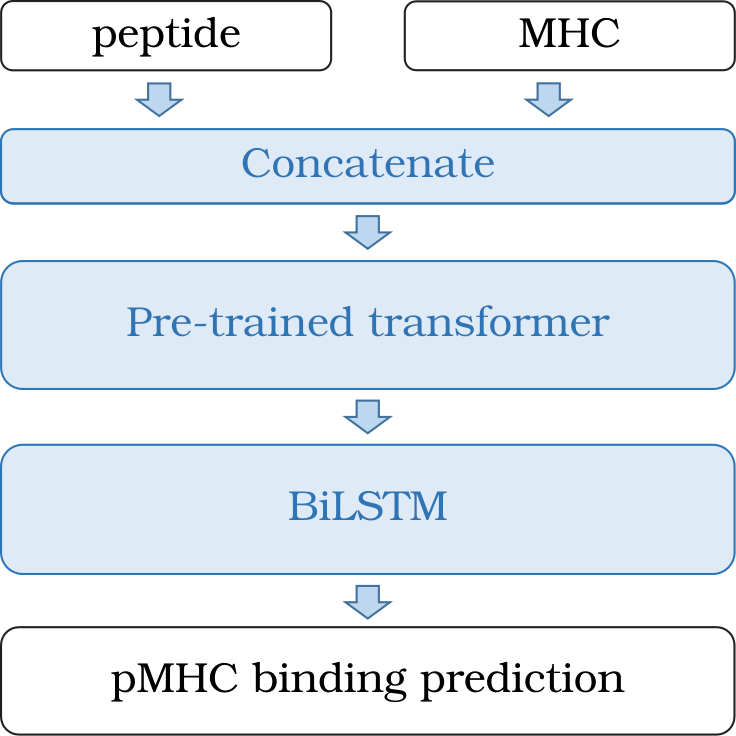
\includegraphics[width=0.7\textwidth]{img/neoantigen/fine_tune2}
		\caption{Transformer model.}
		\label{fig:finetune}
	\end{subfigure}
	\hfill
	\begin{subfigure}[b]{0.56\textwidth}
		\centering
		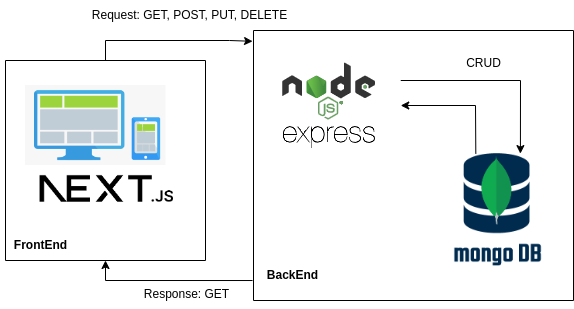
\includegraphics[width=\textwidth]{img/neoantigen/web_arch}
		\caption{Web platform architecture.}
		\label{fig:three sin x}
	\end{subfigure}
	
	\caption{(a) The proposed model for PPI prediction of peptides and MHC. (b) The Web architecture.}
	\label{fig:web}
\end{figure}




\section{Infrastructure}
\section{Limitations}

\section{Expected results and their impact}

\section{Ethics}

\section{Gantt chart}


	
	

\clearpage
	
	%\bibliographystyle{apalike}
	\bibliographystyle{IEEEtran}
	\bibliography{bibliography}
	
\end{document}